\begin{frame}{A Production RAG Pipeline}
  \begin{center}
    \resizebox{\textwidth}{!}{%
    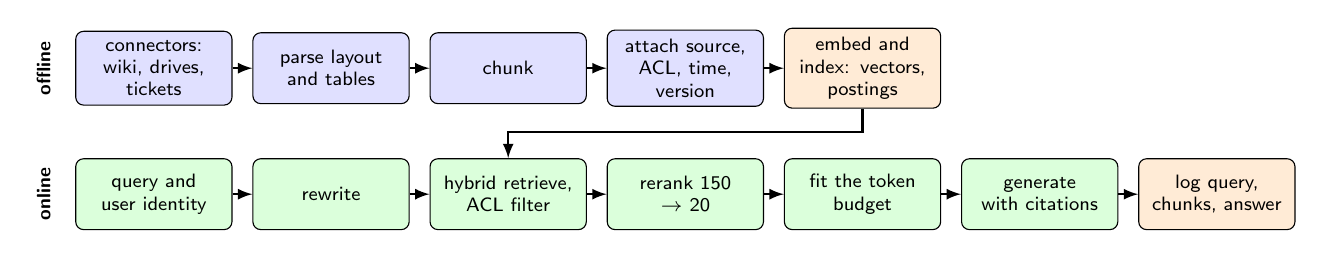
\begin{tikzpicture}[font=\sffamily\scriptsize, >=latex,
        box/.style={draw, rounded corners=0.1cm, align=center, text width=1.75cm, minimum height=0.9cm},
        ofl/.style={box, fill=blue!12}, onl/.style={box, fill=green!14}, sto/.style={box, fill=orange!16},
        arr/.style={->, thick}]
      \node[rotate=90] at (-1.4,1.6) {\textbf{offline}};
      \node[rotate=90] at (-1.4,0) {\textbf{online}};
      \node[ofl] (src)   at (0,1.6)     {connectors: wiki, drives, tickets};
      \node[ofl] (parse) at (2.25,1.6)  {parse layout and tables};
      \node[ofl] (chunk) at (4.5,1.6)   {chunk};
      \node[ofl] (meta)  at (6.75,1.6)  {attach source, ACL, time, version};
      \node[sto] (idx)   at (9.0,1.6)   {embed and index: vectors, postings};
      \node[onl] (q)     at (0,0)       {query and user identity};
      \node[onl] (rw)    at (2.25,0)    {rewrite};
      \node[onl] (ret)   at (4.5,0)     {hybrid retrieve, ACL filter};
      \node[onl] (rr)    at (6.75,0)    {rerank 150 $\to$ 20};
      \node[onl] (asm)   at (9.0,0)     {fit the token budget};
      \node[onl] (gen)   at (11.25,0)   {generate with citations};
      \node[sto] (log)   at (13.5,0)    {log query, chunks, answer};
      \draw[arr] (src) -- (parse);
      \draw[arr] (parse) -- (chunk);
      \draw[arr] (chunk) -- (meta);
      \draw[arr] (meta) -- (idx);
      \draw[arr] (q) -- (rw);
      \draw[arr] (rw) -- (ret);
      \draw[arr] (ret) -- (rr);
      \draw[arr] (rr) -- (asm);
      \draw[arr] (asm) -- (gen);
      \draw[arr] (gen) -- (log);
      \draw[arr] (idx.south) -- ++(0,-0.3) -| (ret.north);
    \end{tikzpicture}}\\[0.3em]
    {\scriptsize Offline, documents become indexed chunks that carry their metadata. Online, each query is rewritten, retrieved under the user's permissions, reranked and packed into the prompt.\par}
  \end{center}
  \vspace{-0.4em}
  \begin{itemize}\footnotesize\itemsep0.3em
    \item[\textcolor{red}{$\blacktriangleright$}] \textbf{Metadata travels with every chunk:} the ACL (access control list: who may read the source) filters retrieval; source and version make citations checkable; the timestamp drives freshness; the embedding-model version says when to re-embed.
    \item[\textcolor{red}{$\blacktriangleright$}] \textbf{A funnel:} Anthropic's tests fetch 150 candidates with embeddings and BM25, rerank them, and pass the top 20 to the model; 20 chunks did better than 5 or 10.
    \item[\textcolor{red}{$\blacktriangleright$}] \textbf{Covered elsewhere:} parsing (document intelligence section), query rewriting and retrieval metrics (covered earlier), citations (hallucination section).
  \end{itemize}
  \vspace{0.1em}
  {\scriptsize Anthropic, ``Introducing Contextual Retrieval,'' 19 Sept.\ 2024, \href{https://www.anthropic.com/news/contextual-retrieval}{anthropic.com/news/contextual-retrieval}.\par}
\end{frame}

\begin{frame}{Chunking: Size, Structure, and Late Chunking}
  \begin{columns}[T,onlytextwidth]
    \column{0.55\textwidth}
      \begin{itemize}\scriptsize\itemsep0.45em
        \item[\textcolor{red}{$\blacktriangleright$}] \textbf{Chunking:} splitting documents into the units that are embedded, retrieved and cited. Small chunks match sharply but lose context (``its'', ``the company''); large ones blur topics into one vector and spend prompt tokens.
        \item[\textcolor{red}{$\blacktriangleright$}] \textbf{Fixed-size:} a set number of tokens, often with a small overlap. Cheap, but it cuts through tables and sections.
        \item[\textcolor{red}{$\blacktriangleright$}] \textbf{Structure-aware:} start a chunk at each title and keep each table whole. On 141 FinanceBench questions over 80 financial reports, element-based chunks reached 53.2\% answer accuracy, against 48.2\% for 512-token and 35.5\% for 128-token chunks, with no chunk size to tune.
        \item[\textcolor{red}{$\blacktriangleright$}] \textbf{Semantic:} cut where the embedding distance between adjacent sentences jumps. Over document retrieval, evidence retrieval and answer generation, its cost was ``not justified by consistent performance gains''; fixed-size chunks won on 3 of 5 evidence-retrieval datasets.
      \end{itemize}
    \column{0.43\textwidth}
      {\centering
      \resizebox{\linewidth}{!}{%
      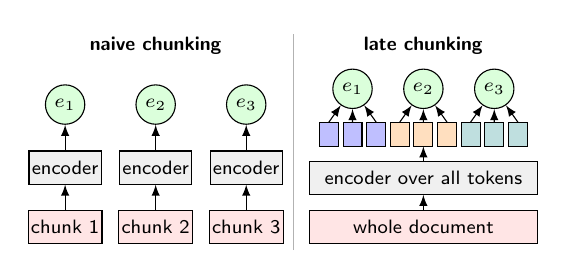
\begin{tikzpicture}[font=\sffamily\scriptsize, >=latex,
          ck/.style={draw, fill=red!10, minimum width=0.8cm, minimum height=0.42cm, inner sep=1pt},
          en/.style={draw, fill=gray!12, minimum height=0.42cm, inner sep=1pt},
          em/.style={draw, circle, fill=green!14, inner sep=1pt, minimum size=0.5cm},
          tk/.style={draw, minimum width=0.24cm, minimum height=0.3cm, inner sep=0pt}]
        \node at (1.65,2.3) {\textbf{naive chunking}};
        \foreach \px/\nm in {0.5/1, 1.65/2, 2.8/3} {
          \node[ck] (c\nm) at (\px,0) {chunk \nm};
          \node[en, minimum width=0.8cm] (n\nm) at (\px,0.75) {encoder};
          \node[em] (e\nm) at (\px,1.55) {$e_{\nm}$};
          \draw[->] (c\nm) -- (n\nm);
          \draw[->] (n\nm) -- (e\nm);
        }
        \node at (5.05,2.3) {\textbf{late chunking}};
        \node[draw, fill=red!10, minimum width=2.9cm, minimum height=0.42cm] (doc) at (5.05,0) {whole document};
        \node[en, minimum width=2.9cm] (enc) at (5.05,0.62) {encoder over all tokens};
        \foreach \tn/\tcol in {1/blue, 2/blue, 3/blue, 4/orange, 5/orange, 6/orange, 7/teal, 8/teal, 9/teal} {
          \node[tk, fill=\tcol!25] (t\tn) at ({3.85+(\tn-1)*0.3},1.17) {};
        }
        \node[em] (l1) at (4.15,1.75) {$e_1$};
        \node[em] (l2) at (5.05,1.75) {$e_2$};
        \node[em] (l3) at (5.95,1.75) {$e_3$};
        \draw[->] (doc) -- (enc);
        \draw[->] (enc) -- (5.05,1.02);
        \foreach \tn in {1,2,3} {\draw[->] (t\tn.north) -- (l1);}
        \foreach \tn in {4,5,6} {\draw[->] (t\tn.north) -- (l2);}
        \foreach \tn in {7,8,9} {\draw[->] (t\tn.north) -- (l3);}
        \draw[gray!60] (3.4,-0.3) -- (3.4,2.45);
      \end{tikzpicture}}\\[0.2em]
      {\scriptsize Redrawn after G\"unther et al., ``Late Chunking: Contextual Chunk Embeddings Using Long-Context Embedding Models,'' 2024, \href{https://arxiv.org/abs/2409.04701v1}{arXiv:2409.04701v1}, Figure~2.\par}\par}
      \begin{itemize}\scriptsize
        \item[\textcolor{red}{$\blacktriangleright$}] \textbf{Late chunking:} encode the whole document once with a long-context model (8{,}192 tokens), then mean-pool each chunk's token vectors, so $e_2$ also depends on chunks 1 and 3. With 256-token chunks, nDCG@10 rose from 23.5 to 30.0 on NFCorpus and from 64.2 to 66.1 on SciFact.
      \end{itemize}
  \end{columns}
  \vspace{0.1em}
  {\scriptsize Jimeno Yepes et al., ``Financial Report Chunking for Effective Retrieval Augmented Generation,'' \href{https://arxiv.org/abs/2402.05131v3}{arXiv:2402.05131v3}, Table~5; Qu, Tu and Bao, ``Is Semantic Chunking Worth the Computational Cost?,'' \href{https://arxiv.org/abs/2410.13070v1}{arXiv:2410.13070v1}, Table~2; late-chunking numbers from G\"unther et al., Table~2.\par}
\end{frame}

\begin{frame}{Contextual Retrieval and HyDE}
  \begin{columns}[T,onlytextwidth]
    \column{0.52\textwidth}
      \begin{itemize}\scriptsize\itemsep0.3em
        \item[\textcolor{red}{$\blacktriangleright$}] \textbf{Contextual retrieval:} at ingestion an LLM (Claude 3 Haiku in the post) reads the whole document and writes 50--100 tokens that situate each chunk, prepended before embedding (Anthropic's \textbf{contextual embeddings}, unrelated to the contextual word vectors covered earlier) and before BM25 indexing (\textbf{contextual BM25}).
        \item[\textcolor{red}{$\blacktriangleright$}] \textbf{Example:} ``The company's revenue grew by 3\% over the previous quarter.'' names no company and no date; the prefix adds ACME, Q2 2023 and the previous quarter's revenue.
      \end{itemize}
      \vspace{0.2em}
      {\centering\scriptsize Failed retrievals in the top 20 ($1 - \text{recall@20}$), Gemini Text 004 embeddings, mean of five evaluation sets:\\[0.15em]
      \begin{tabular}{lcc}
        \toprule
        chunks & standard & contextual \\
        \midrule
        embeddings & 5.7\% & 3.7\% \\
        + BM25, fused & 5.0\% & 2.9\% \\
        + rerank 150 $\to$ 20 & 3.5\% & 1.9\% \\
        \bottomrule
      \end{tabular}\par}
      \vspace{0.2em}
      \begin{itemize}\scriptsize
        \item[\textcolor{red}{$\blacktriangleright$}] \textbf{Cost:} one LLM call per chunk, once. With the document in the prompt cache (prefix caching, covered earlier): \$1.02 per million document tokens, for 8k-token documents and 800-token chunks.
      \end{itemize}
    \column{0.46\textwidth}
      \begin{itemize}\scriptsize
        \item[\textcolor{red}{$\blacktriangleright$}] \textbf{HyDE} (hypothetical document embeddings): an instruction-following LLM writes a passage that would answer the query, a contrastively trained encoder embeds it, and search returns the real documents nearest to it. The encoder's ``dense bottleneck'' drops most of what the passage invents.
      \end{itemize}
      \vspace{0.2em}
      {\centering
      \resizebox{\linewidth}{!}{%
      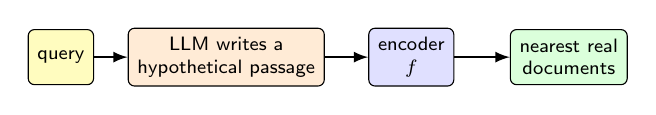
\begin{tikzpicture}[font=\sffamily\scriptsize, >=latex,
          hb/.style={draw, rounded corners=0.08cm, align=center, minimum height=0.7cm}]
        \node[hb, fill=yellow!25] (q) at (0,0) {query};
        \node[hb, fill=orange!16] (g) at (2.1,0) {LLM writes a\\hypothetical passage};
        \node[hb, fill=blue!12] (e) at (4.45,0) {encoder\\$f$};
        \node[hb, fill=green!14] (r) at (6.45,0) {nearest real\\documents};
        \draw[->, thick] (q) -- (g);
        \draw[->, thick] (g) -- (e);
        \draw[->, thick] (e) -- (r);
      \end{tikzpicture}}\par}
      \begin{itemize}\scriptsize\itemsep0.3em
        \item[\textcolor{red}{$\blacktriangleright$}] Query vector from $N$ generated passages $\hat{d}_k$ and the query $q$, with encoder $f$:
          \[ \hat{v}_q = \frac{1}{N+1}\Big[\sum_{k=1}^{N} f(\hat{d}_k) + f(q)\Big] \]
        \item[\textcolor{red}{$\blacktriangleright$}] With no relevance labels, nDCG@10 on TREC DL19 (web queries over MS MARCO) rose from 44.5 for the encoder alone to 61.3, above BM25 (50.6) and close to DPR fine-tuned on MS MARCO (62.2). The price: one LLM generation before every search.
      \end{itemize}
  \end{columns}
  \vspace{0.1em}
  {\scriptsize Contextual retrieval: Anthropic (2024), text and charts. Gao et al., ``Precise Zero-Shot Dense Retrieval without Relevance Labels,'' ACL 2023, \href{https://aclanthology.org/2023.acl-long.99/}{aclanthology.org/2023.acl-long.99}, Section~3, Eq.~8, Table~1.}
\end{frame}

\begin{frame}{Permission-Aware Retrieval}
  \begin{columns}[T,onlytextwidth]
    \column{0.47\textwidth}
      {\centering
      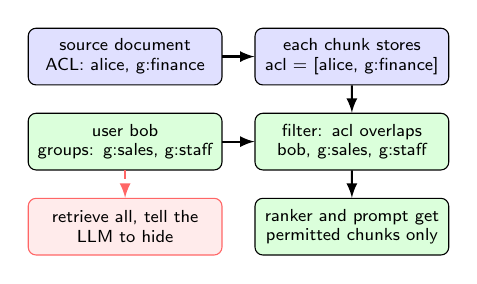
\begin{tikzpicture}[font=\sffamily\scriptsize, >=latex, scale=0.9, every node/.style={transform shape},
          box/.style={draw, rounded corners=0.1cm, align=center, text width=2.5cm, minimum height=0.8cm},
          ing/.style={box, fill=blue!12}, qry/.style={box, fill=green!14}, bad/.style={box, fill=red!8, draw=red!60}]
        \node[ing] (src)  at (0,2.3)   {source document\\ACL: alice, g:finance};
        \node[ing] (meta) at (3.2,2.3) {each chunk stores\\acl = [alice, g:finance]};
        \node[qry] (user) at (0,1.1)   {user bob\\groups: g:sales, g:staff};
        \node[qry] (flt)  at (3.2,1.1) {filter: acl overlaps\\bob, g:sales, g:staff};
        \node[bad] (llm)  at (0,-0.1)  {retrieve all, tell the\\LLM to hide \xmark};
        \node[qry] (ok)   at (3.2,-0.1){ranker and prompt get\\permitted chunks only};
        \draw[->, thick] (src) -- (meta);
        \draw[->, thick] (meta) -- (flt);
        \draw[->, thick] (user) -- (flt);
        \draw[->, thick] (flt) -- (ok);
        \draw[->, thick, dashed, red!60] (user) -- (llm);
      \end{tikzpicture}\\[0.2em]
      {\scriptsize The ACL is copied at ingestion and applied as a filter inside retrieval, so the model never receives a chunk the user could not open.\par}\par}
      \vspace{0.3em}
      \begin{itemize}\scriptsize
        \item[\textcolor{red}{$\blacktriangleright$}] \textbf{Oversharing:} trimming reproduces the source permissions, mistakes included. A file shared with everyone becomes retrievable by everyone, and the assistant will find it (the copilots section returns to oversharing).
      \end{itemize}
    \column{0.51\textwidth}
      \begin{itemize}\scriptsize\itemsep0.4em
        \item[\textcolor{red}{$\blacktriangleright$}] \textbf{ACL} (access control list): the users and groups allowed to read a document, kept by its source system. Ingestion copies each document's ACL into the metadata of all its chunks.
        \item[\textcolor{red}{$\blacktriangleright$}] \textbf{Security trimming:} every query carries the user's identities as a filter, so a chunk the user cannot open never reaches the ranker or the prompt. In Azure AI Search's security-filter pattern, for setups that cannot use its built-in ACL support, the filter matches group IDs stored as strings, with ``no authentication or authorization through the security principal'': the application must authenticate the user and expand their groups.
        \item[\textcolor{red}{$\blacktriangleright$}] \textbf{Never ask the LLM to withhold} what is already in its context: a plain question or a prompt injection (covered earlier) can bring it out. Enforce the filter inside retrieval, and key caches the same way (end of this section).
        \item[\textcolor{red}{$\blacktriangleright$}] \textbf{Propagation:} a revoked share, a deleted file or a changed group membership must reach the index; until it does, the stale ACL decides. Sync permissions from the same change feed as content.
      \end{itemize}
  \end{columns}
  \vspace{0.1em}
  {\scriptsize Microsoft, ``Security filters for trimming results in Azure AI Search,'' Microsoft Learn, updated Aug.\ 2026, \href{https://learn.microsoft.com/en-us/azure/search/search-security-trimming-for-azure-search}{learn.microsoft.com/en-us/azure/search}.}
\end{frame}

\begin{frame}{Multi-Tenancy and Index Freshness}
  \begin{columns}[T,onlytextwidth]
    \column{0.50\textwidth}
      \begin{itemize}\scriptsize
        \item[\textcolor{red}{$\blacktriangleright$}] \textbf{Multi-tenancy:} one deployment serves several customers or business units whose data must never mix. In Qdrant ``each collection carries its own resource overhead'', which sets the layout:
      \end{itemize}
      \vspace{0.2em}
      {\centering\scriptsize\setlength{\tabcolsep}{4pt}
      \begin{tabular}{lll}
        \toprule
        \textbf{Layout} & \textbf{Isolation} & \textbf{Suits} \\
        \midrule
        collection per tenant & strict & few tenants \\
        shared, tenant filter & by filter & many small tenants \\
        shard per tenant & strong & a few large tenants \\
        \bottomrule
      \end{tabular}\par}
      \vspace{0.3em}
      \begin{itemize}\scriptsize\itemsep0.4em
        \item[\textcolor{red}{$\blacktriangleright$}] \textbf{Shared statistics:} in a shared collection, BM25's $N$ and $n_t$ count every tenant, ``so a term's IDF no longer reflects its rarity within a specific tenant's data''. Scope them per tenant where the engine allows.
        \item[\textcolor{red}{$\blacktriangleright$}] \textbf{Selective filters:} a small tenant or a narrow ACL passes a tiny fraction of the index, the hard case for post-filtering (see the semantic search section). Measure recall under the tightest real filters.
      \end{itemize}
    \column{0.48\textwidth}
      \begin{itemize}\scriptsize\itemsep0.4em
        \item[\textcolor{red}{$\blacktriangleright$}] \textbf{Incremental ingestion:} read each source's change feed (created, updated, deleted, re-permissioned), re-parse and re-embed only what changed, and stamp each chunk with the source version.
        \item[\textcolor{red}{$\blacktriangleright$}] \textbf{Deletes in graph indexes:} an HNSW node (covered in the CV course) lies on many search paths, and Faiss's HNSW index ``does not support removing vectors from the index''. FreshDiskANN keeps a deleted node in the graph to route searches, filters it out of results, and repairs the graph in batches once 1--10\% of the points are deleted. Until the repair, that result filter alone hides the deleted text.
        \item[\textcolor{red}{$\blacktriangleright$}] \textbf{Rebuilds are slow:} a good HNSW index over 100M points takes about 1.5--2 hours on a dedicated 48-core machine, so freshness by periodic rebuild is expensive.
      \end{itemize}
  \end{columns}
  \vspace{0.1em}
  {\scriptsize Qdrant documentation, ``Multitenancy,'' \href{https://qdrant.tech/documentation/guides/multiple-partitions/}{qdrant.tech/documentation/guides/multiple-partitions}. Faiss wiki, ``Guidelines to choose an index,'' \href{https://github.com/facebookresearch/faiss/wiki/Guidelines-to-choose-an-index}{github.com/facebookresearch/faiss/wiki}. Singh et al., ``FreshDiskANN: A Fast and Accurate Graph-Based ANN Index for Streaming Similarity Search,'' 2021, \href{https://arxiv.org/abs/2105.09613v1}{arXiv:2105.09613v1}, Sections~1, 3.3, 4.2.}
\end{frame}

\begin{frame}{Re-Embedding and Caching}
  \begin{itemize}\footnotesize
    \item[\textcolor{red}{$\blacktriangleright$}] \textbf{A new embedding model means a new index:} vectors from two models live in different spaces. Re-embed into a versioned index, switch once it passes the retrieval evaluation (covered earlier), and keep the old one for rollback.
  \end{itemize}
  \vspace{0.1em}
  {\centering\scriptsize
  \begin{tabular}{llll}
    \toprule
    \textbf{Cache} & \textbf{Key} & \textbf{Reused on} & \textbf{Main risk} \\
    \midrule
    exact response & query, permissions, index version & same request & stale after an update \\
    prefix (covered earlier) & token prefix & same prefix & none to correctness \\
    semantic & query embedding, permissions & similar query & answers another question \\
    \bottomrule
  \end{tabular}\par}
  \vspace{0.2em}
  \begin{itemize}\footnotesize\itemsep0.3em
    \item[\textcolor{red}{$\blacktriangleright$}] \textbf{Semantic cache:} returns a stored answer when a new query's embedding is close to a cached one. GPTCache answers 2--10$\times$ faster on a hit, yet in its own test 39 of 876 hits (4.5\%) returned an answer cached for a dissimilar question.
    \item[\textcolor{red}{$\blacktriangleright$}] \textbf{Key on permissions:} an answer built from documents Alice can read must never reach Bob. Put the permission set and index version in every key; invalidate on document and ACL changes.
    \item[\textcolor{red}{$\blacktriangleright$}] \textbf{Retrieval or a long window} (covered earlier): by Anthropic's rule of thumb, a knowledge base under about 200K tokens can go straight into the prompt.
  \end{itemize}
  \vspace{0.1em}
  {\scriptsize Fu and Feng, ``GPTCache,'' NLP-OSS 2023, \href{https://aclanthology.org/2023.nlposs-1.24/}{aclanthology.org/2023.nlposs-1.24}, Sections~4--5, Table~1; Anthropic (2024), contextual retrieval post.\par}
\end{frame}
